\subsection{Prototype Hardware}
% Add drawings / design philosophy 
The robot is designed with the Open Continuum Robotics project in mind. It uses easily accessible, off-the-shelf components, and 3D printed parts so that other groups can reconstruct the same robot. A full breakdown of the robot's physical design can be found in Appendix \ref{app:robot_drawings}. 

\subsubsection{Physical Description of Prototype}
\label{sec:physical_description}
% Arms
\paragraph{The arms} are each \SI{80}{cm} long and consist of a \SI{0.0200}{"} thick, \SI{0.75}{"} wide beam made from 1095 spring steel, with 19 evenly spaced 3D printed tendon spacers. The spacers hold one tendon on each side of the beam \SI{11}{mm} away from the steel beam. The 1095 spring steel beam is used as the central beam as it provides rigidity in the direction of motion off the robot's planar surface, while remaining flexible along the plane. The high elasticity of the material allows the system to undergo large curvatures without permanently deforming the beam. The tendons used are \SI{30}{lbs} braided fishing line (Super8Slick V2, Power Pro, CA, USA). Each tendon has four \SI{0.75}{"} nuts on it that act to maintain tension during operational periods where it is being extended. 

\begin{figure}[h]
    \centering
    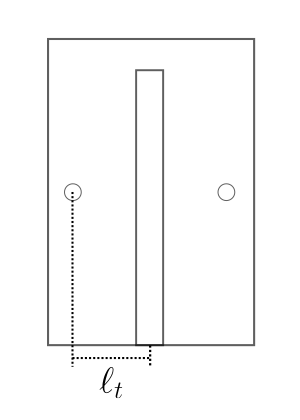
\includegraphics[width=0.3\textwidth]{images/beam_cross_section.png}
    \caption{Cross section of the beam spacers. $\ell_t = \SI{11}{mm}$}
    \label{fig:beam_cross_section}
\end{figure}

\begin{figure}[h]
    \centering
    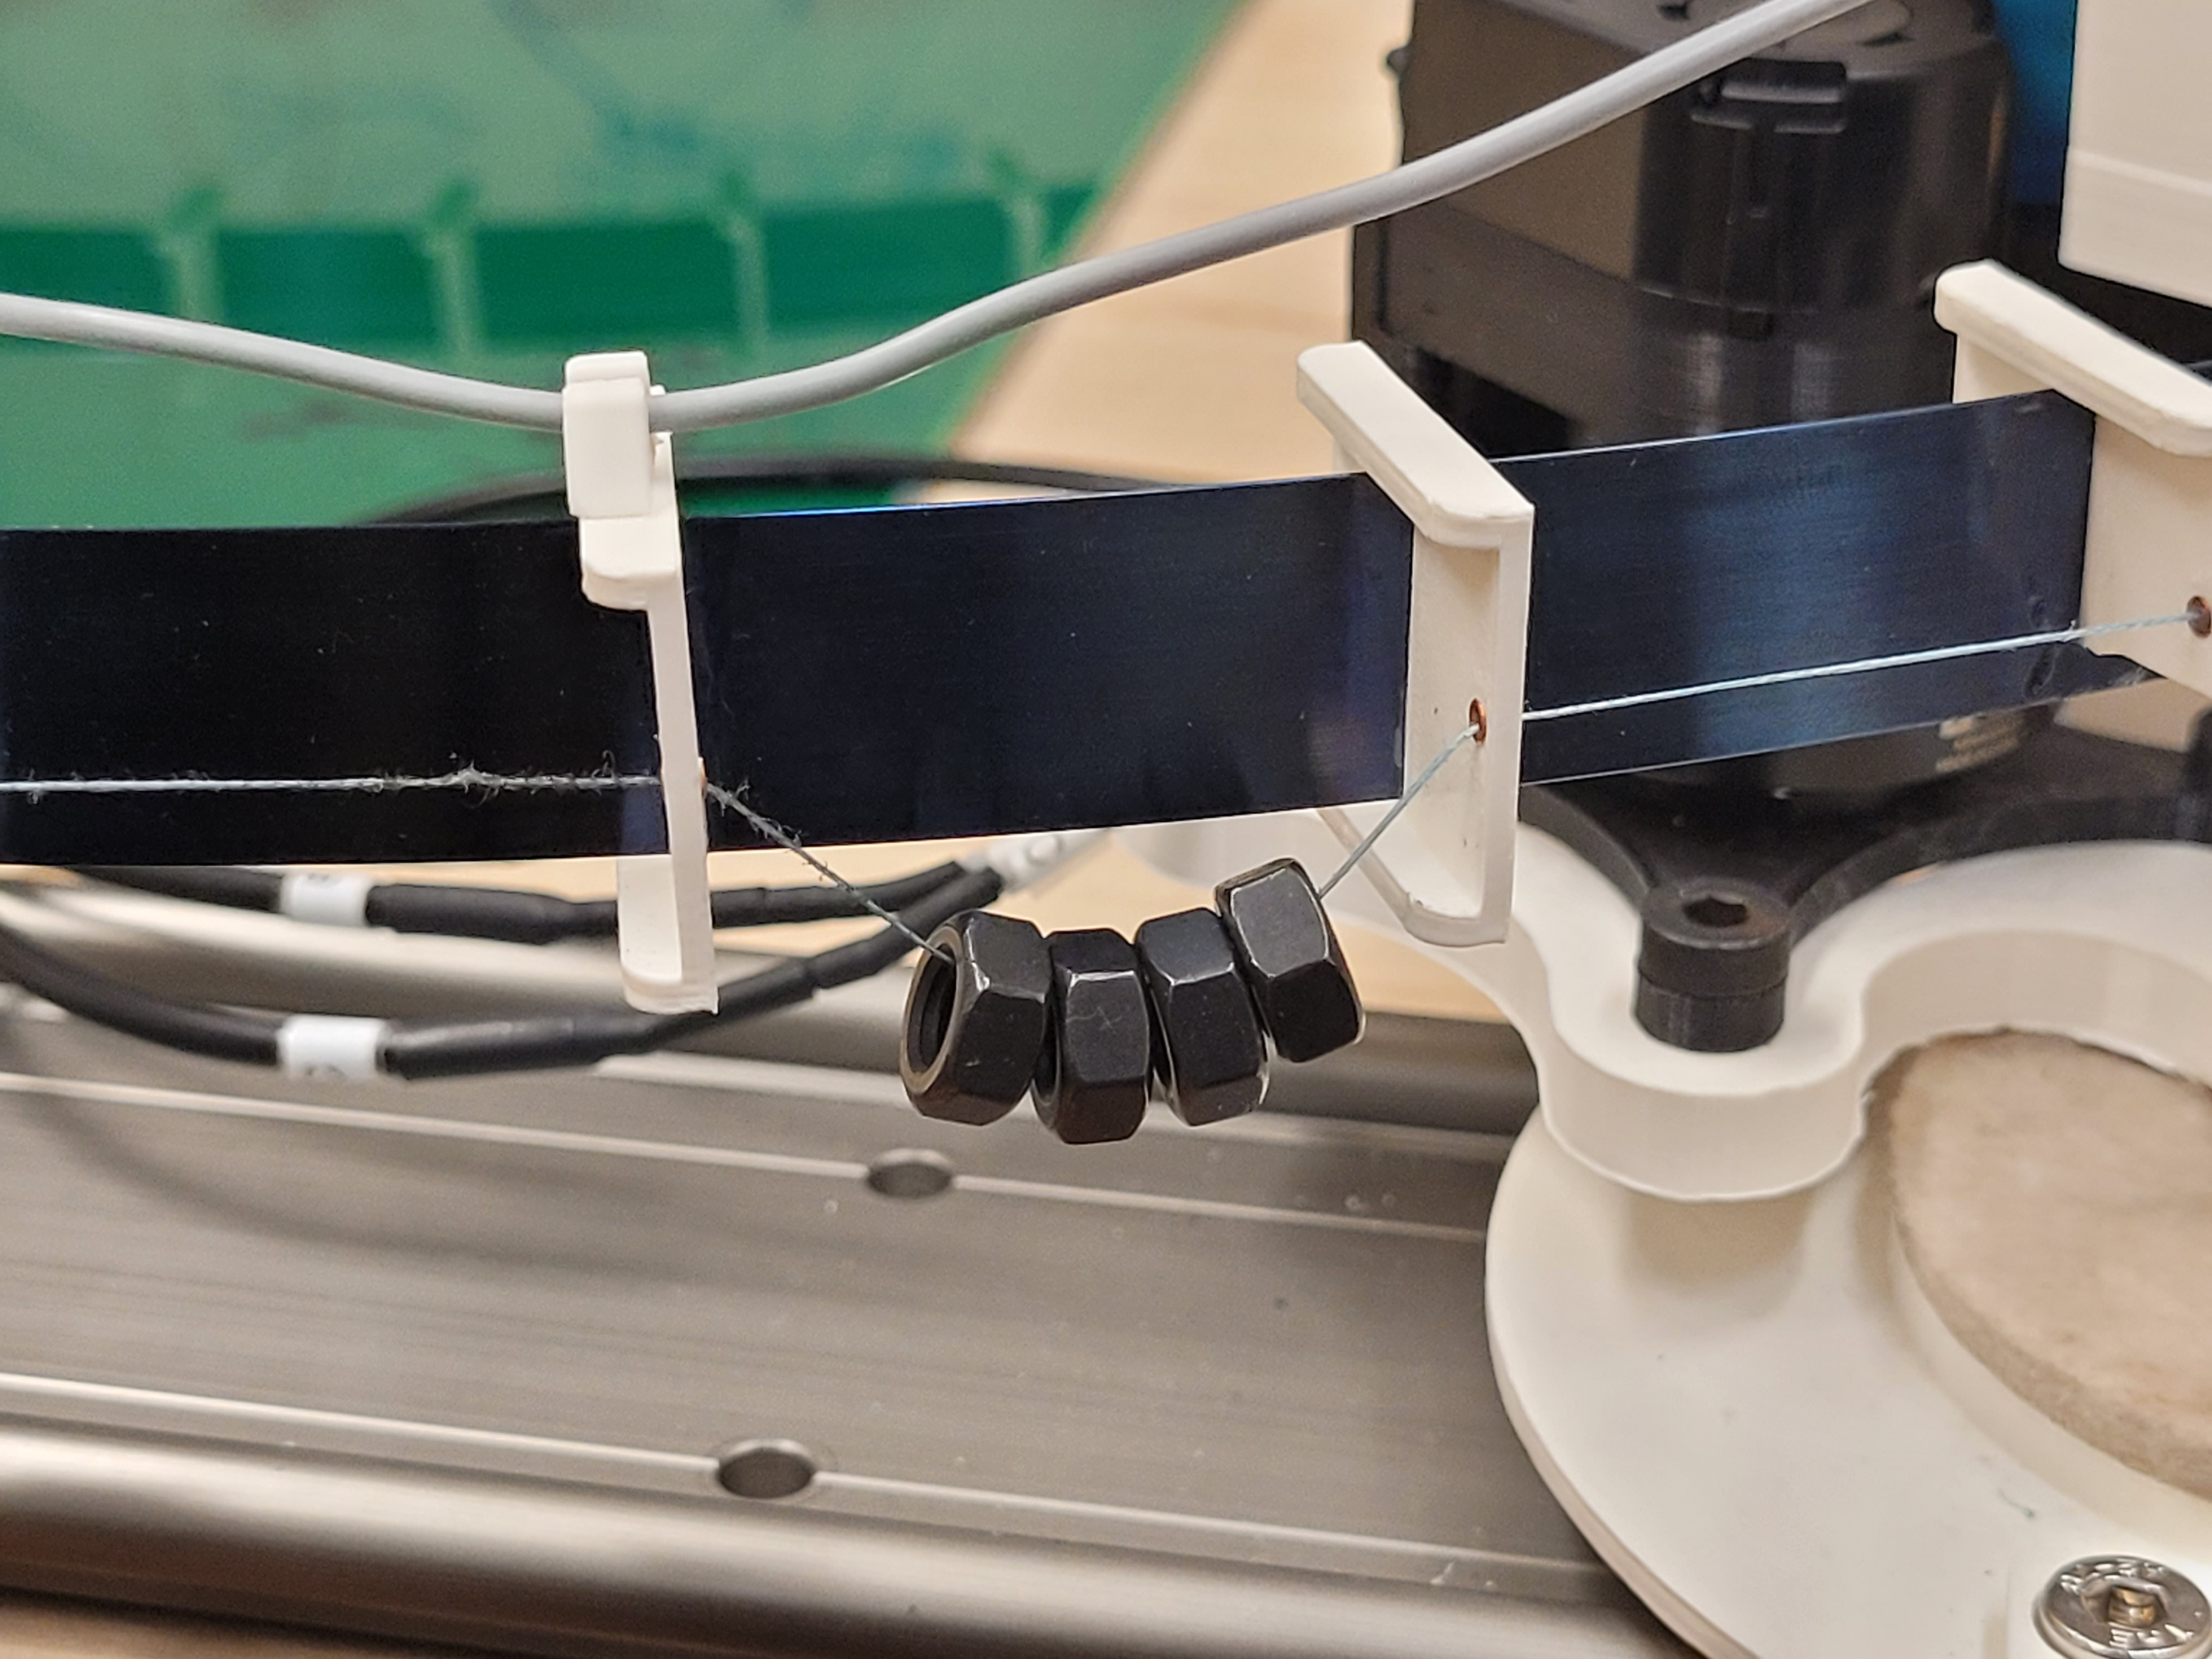
\includegraphics[width=0.5\textwidth]{images/tendon_slack.jpg}
    \caption{Four \SI{0.75}{"} nuts placed on a tendon to maintain tendon tension throughout operation}
    \label{fig:tendon_slack}
\end{figure}

% \begin{figure}[h]
%      \centering
%      \begin{subfigure}[b]{0.48\textwidth}
%          \centering
%          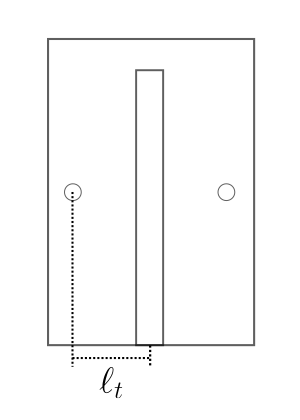
\includegraphics[width=0.625\textwidth]{images/beam_cross_section.png}
%          \caption{Cross section of the beam spacers. $\ell_t = \SI{11}{mm}$}
%          \label{fig:beam_cross_section}
%      \end{subfigure}
%      \hfill
%      \begin{subfigure}[b]{0.48\textwidth}
%          \centering
%          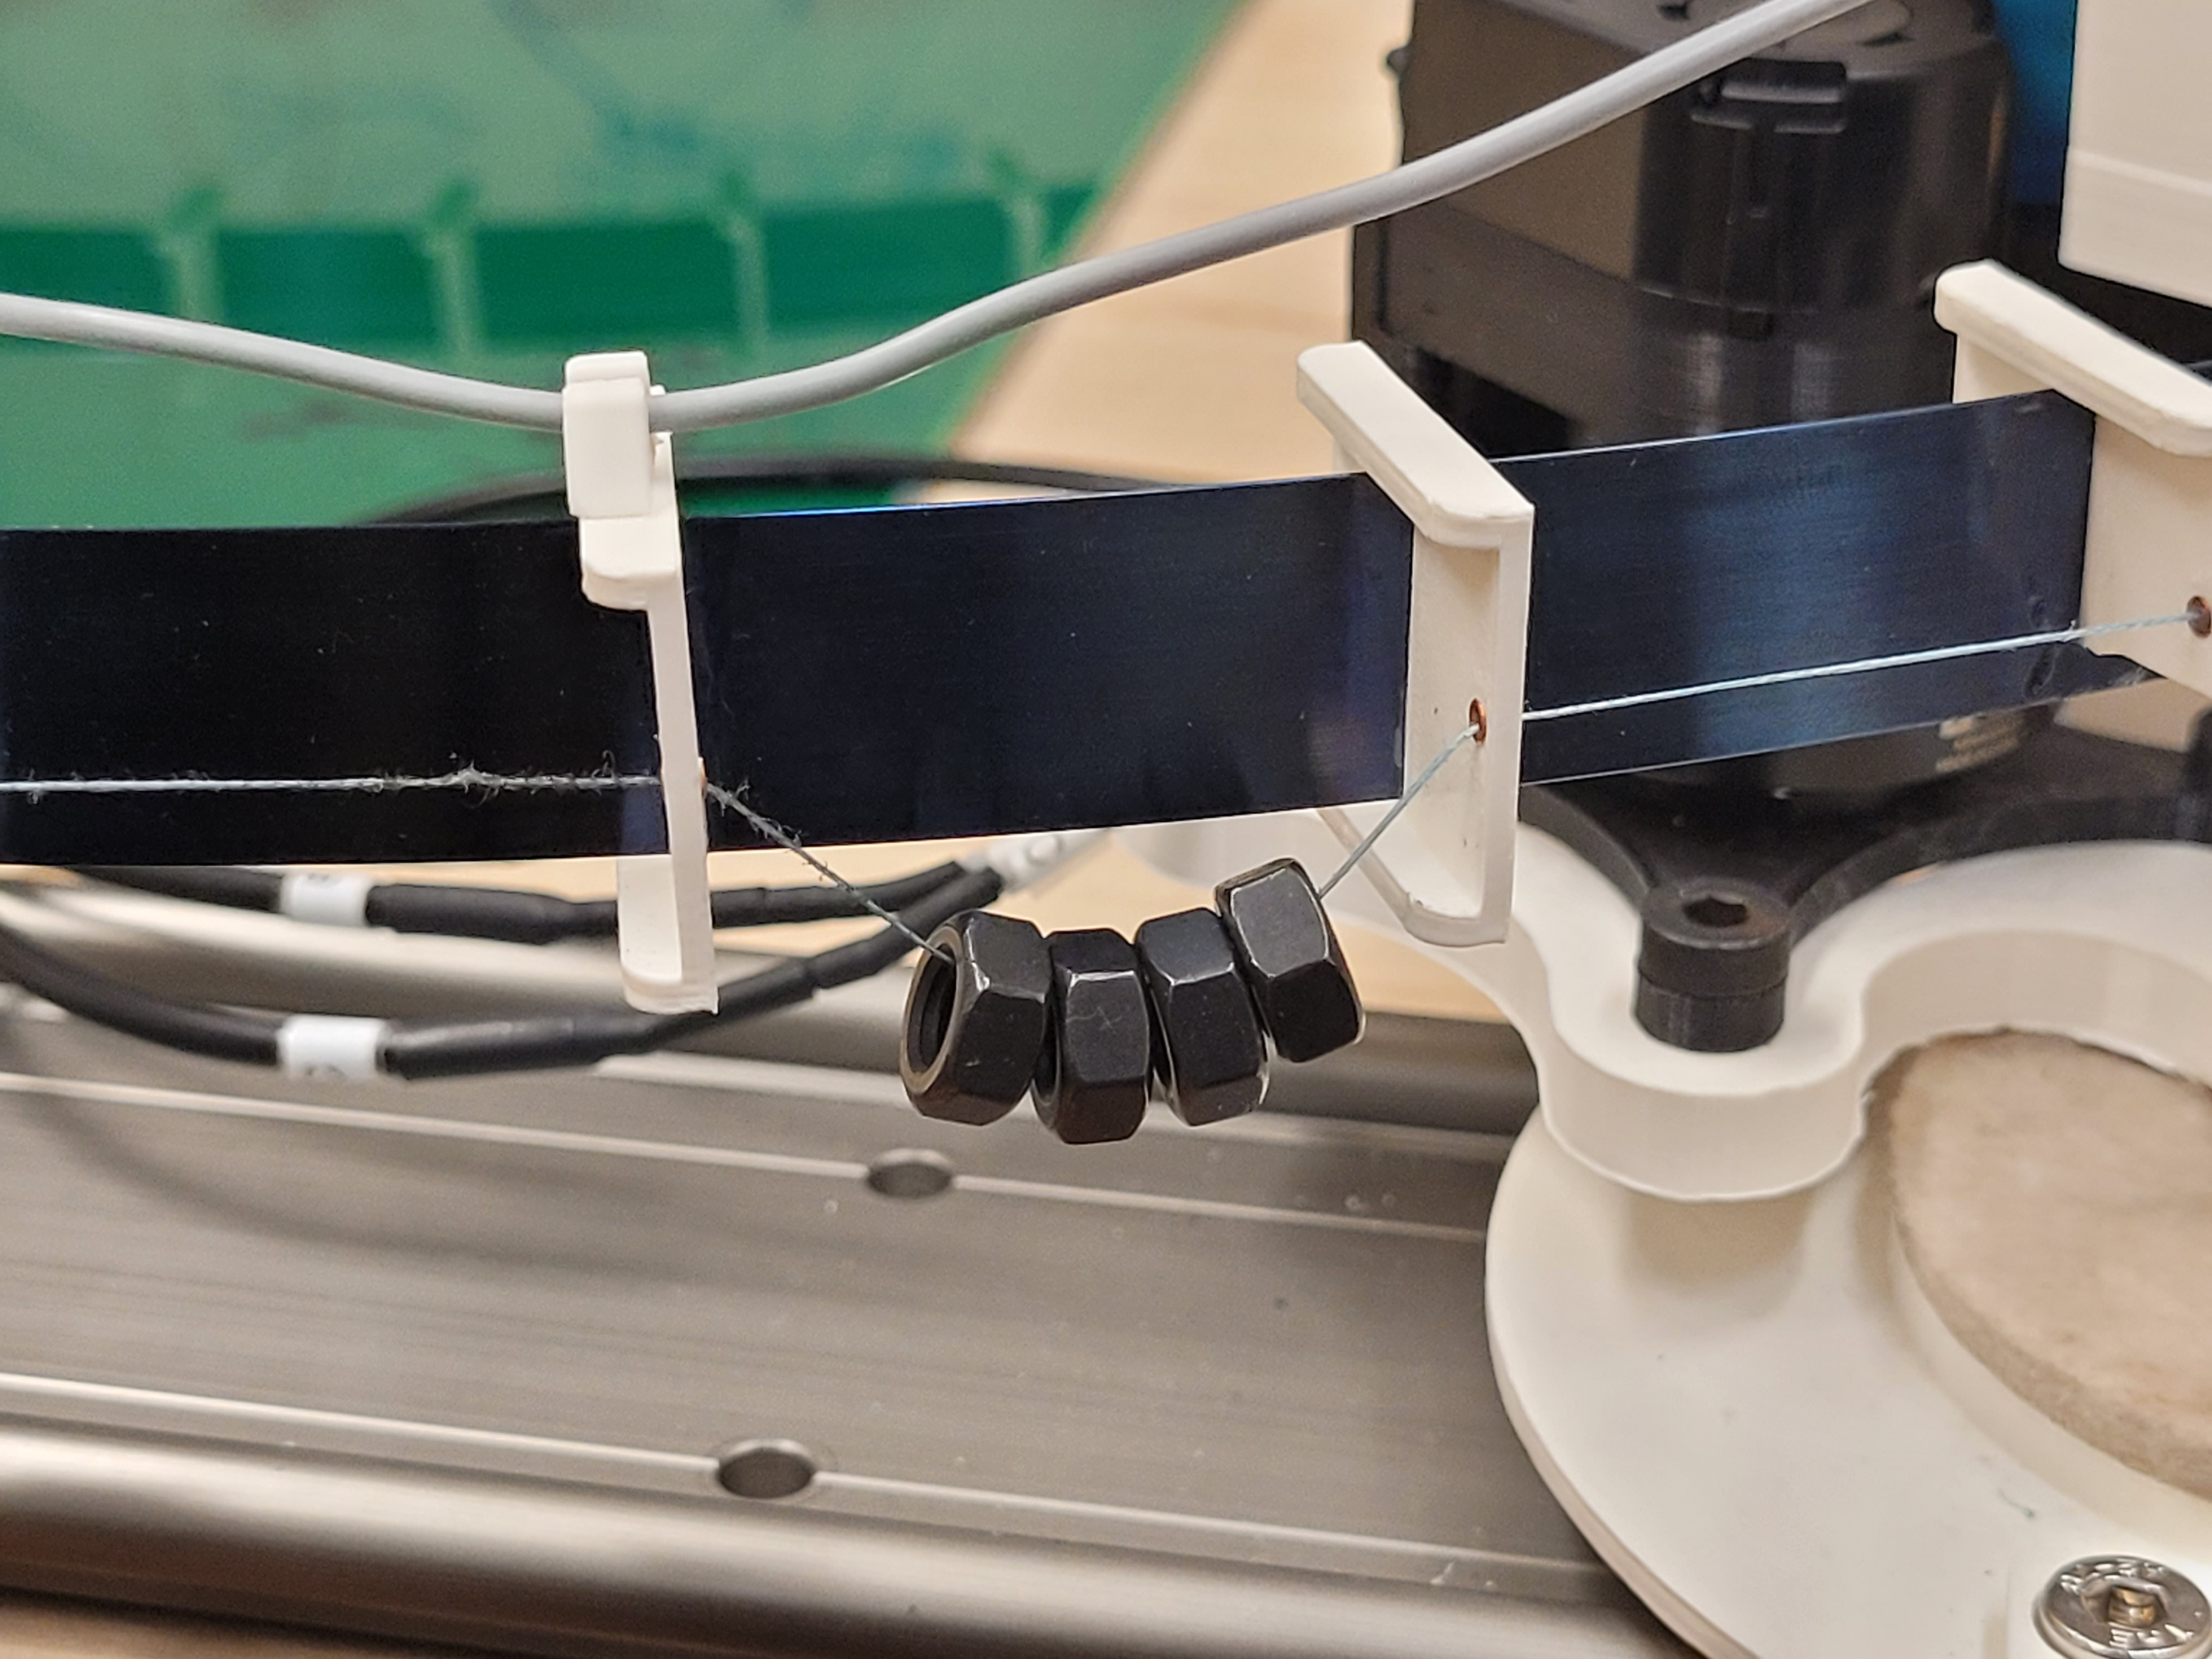
\includegraphics[width=\textwidth]{images/tendon_slack.jpg}
%          \caption{Four \SI{0.75}{"} nuts placed on a tendon to maintain tendon tension throughout operation}
%          \label{fig:tendon_slack}
%      \end{subfigure}
% \end{figure}

% Joints and End Effector  
\paragraph{The end effector} features a wide base to prevent the end effector from twisting off the plane. Revolute joints link the ends of each arm to the motor bases and the end effector, allowing both ends to rotate freely about the z-axis. The two arms share the same end effector. The bases for each arm are positioned \SI{60}{cm} apart.Each arm having its own independent degree of freedom grants the end effector in this configuration two degrees of freedom laying on the table plane. At this distance, the reachable workspace of the end effector covers a majority of the AURORA tracker workspace. During operation, a smaller end effector base does not provide enough area to balance the moments being applied by the two arms actuating the piece from different heights. Figure \ref{fig:ee_comparison} demonstrates this effect in action. Felt pads are attached to the bottom of the end effector to reduce friction between the end effector and table surface. 

\begin{figure}[h]
     \centering
     \begin{subfigure}[b]{0.48\textwidth}
         \centering
         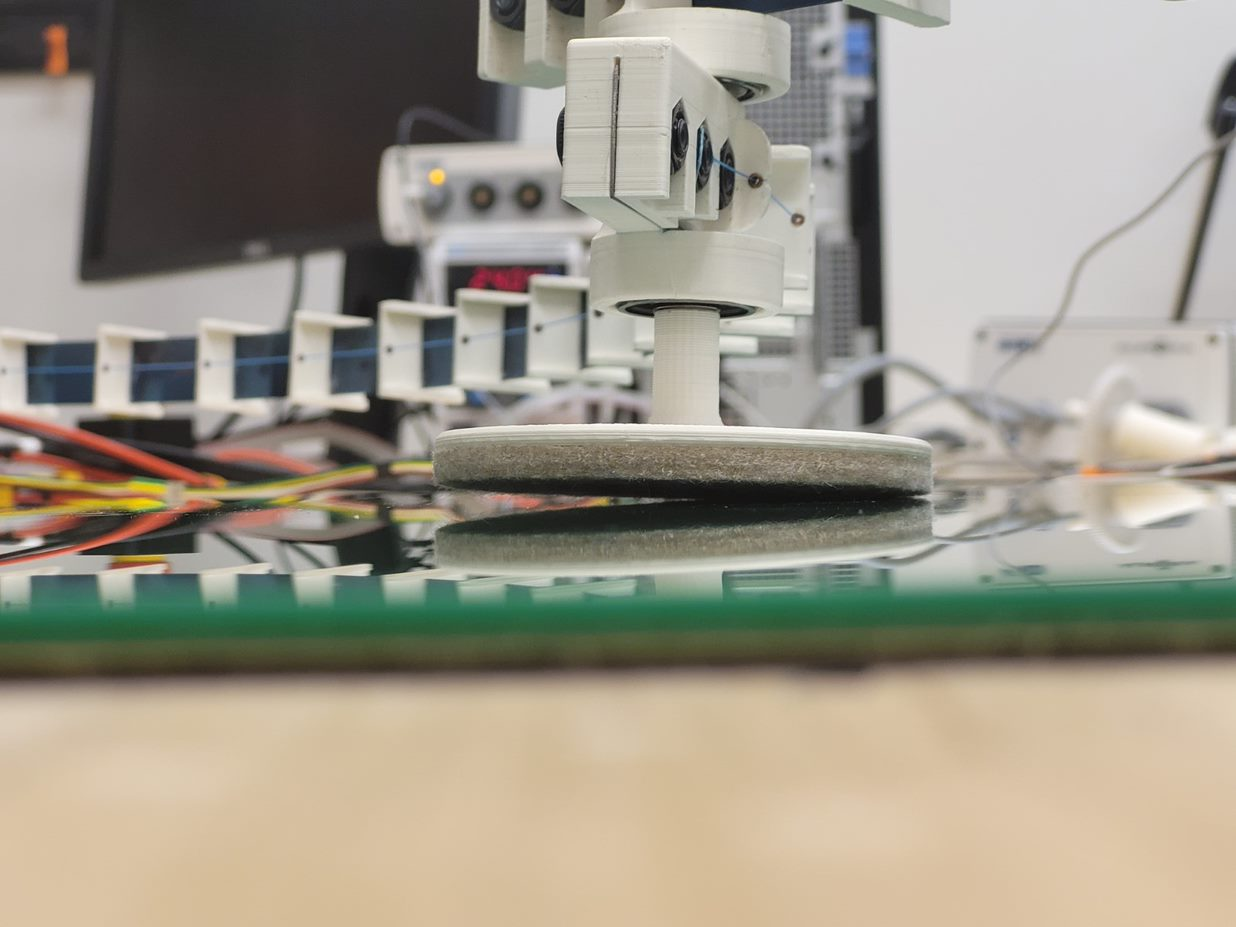
\includegraphics[width=\textwidth]{images/small_ee.jpeg}
         \caption{Smaller base causing the end effector to twist off the planar surface}
         \label{fig:small_ee}
     \end{subfigure}
     \hfill
     \begin{subfigure}[b]{0.48\textwidth}
         \centering
         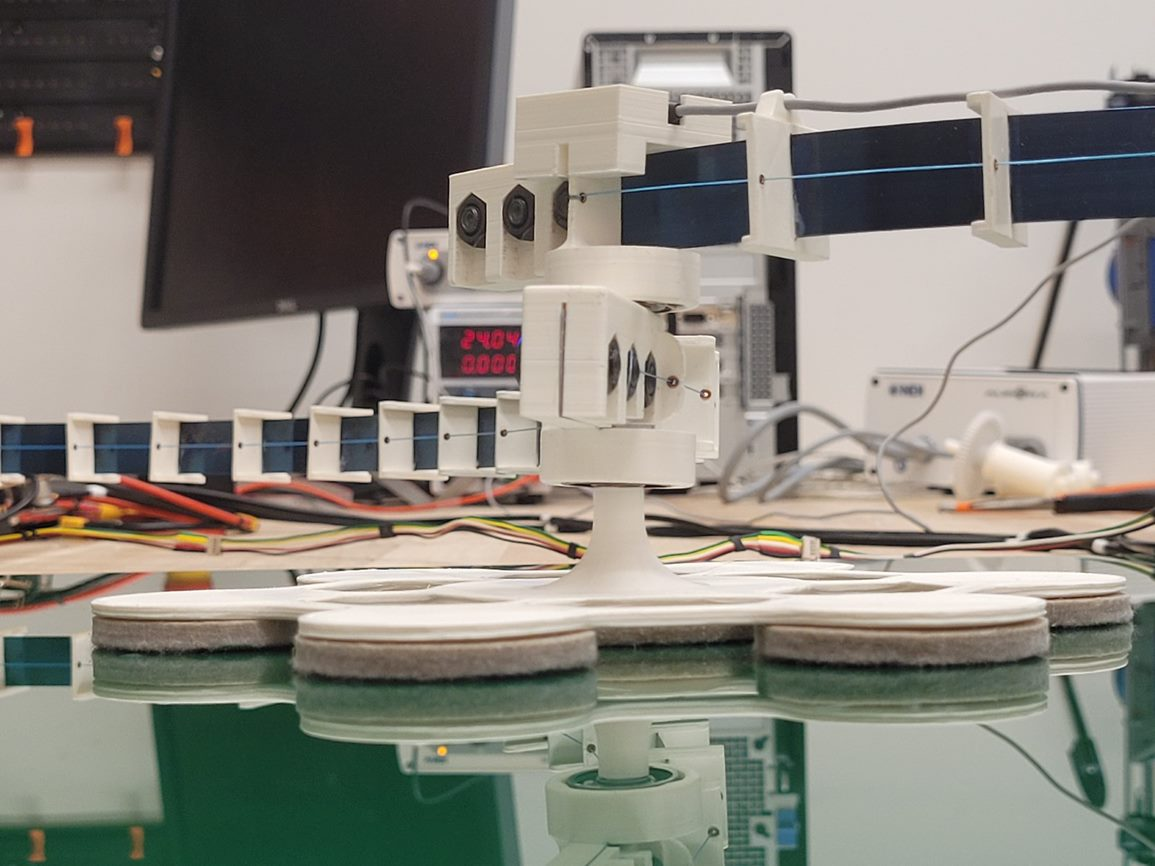
\includegraphics[width=\textwidth]{images/large_ee.jpeg}
         \caption{Larger base ensuring end effector remains on the plane}
         \label{fig:large_ee}
     \end{subfigure}
        \caption{Comparison of end effector sizes}
        \label{fig:ee_comparison}
\end{figure}

\paragraph{Gearboxes} are actuated directly by motors for each arm. The gear boxes are 3D printed but use purchase gears with a gear ratio of 16:1, enabling significantly higher applied torques than the motors are natively capable of. A 4:1 gear ratio is achieved by the motor unit. This results in a total gear ratio of 64:1 for the actuation unit. Each box contains two \SI{10}{mm} gears (2662N313, McMaster-Carr Supply Company, IL, USA) and three \SI{40}{mm} gears (2662N321, McMaster-Carr Supply Company, IL, USA) to achieve this rotation. The gearbox actuates a 3D printed spindle with a radius of \SI{11}{mm}. Two tendons are spooled around the spindle in opposite directions, so when it rotates, one tendon is extended while the other is contracted. Both tendons are firmly attached at the end effector side of each arm. This equal and opposite actuation of the tendons is what causes the arm to bend. 

% Workspace 
\paragraph{The workspace} additionally has an acrylic sheet used to reduce friction. Beneath the table surface, an AURORA electromagnetic tracking system (20-20 planar, Northern Digital Inc., ON, Canada) is positioned. The tracker is positioned to ensure maximal coverage of the robot's task space. The tracker is limited to an effective tracking area of \SI{50}{cm} x \SI{50}{cm} on the workspace plane. This unit tracks a wire coil which is fastened on the robot's end effector, directly above the revolute joint. This is where the end effector position is defined to be as a point in space. 

\subsubsection{Electronic Components}
Each arm is driven by a single Antigravity drone motor (MN4004 KV300, T-MOTOR, JX, P.R. China) which are both controlled by an off-the-shelf microprocessor (LAUNCHXL-F28069M, Texas Instruments, Dallas, USA) fitted with two booster cards (BOOSTXL-DRV8305EVM, Texas Instruments, Dallas, USA). The motors are part of an actuation unit shown in Figure \ref{fig:motor_unit} and contain a 4:1 gear ratio and an Avago optical encoder (AEDM 5810, Broadcom Inc., CA, USA) that is used to provide system feedback at a rate of \SI{1000}{hz} to the workstation. The actuation setup comes from the Open Continuum Robot project \cite{open_cr, Grimminger_2020}. A single micro-controller communicates with a workstation through the CAN bus protocol. The robot is powered using a \SI{240}{W} power supply operating at \SI{24}{V}. An emergency stop is installed within reach of the operator for safety. 

\begin{figure}[p]
    \centering
    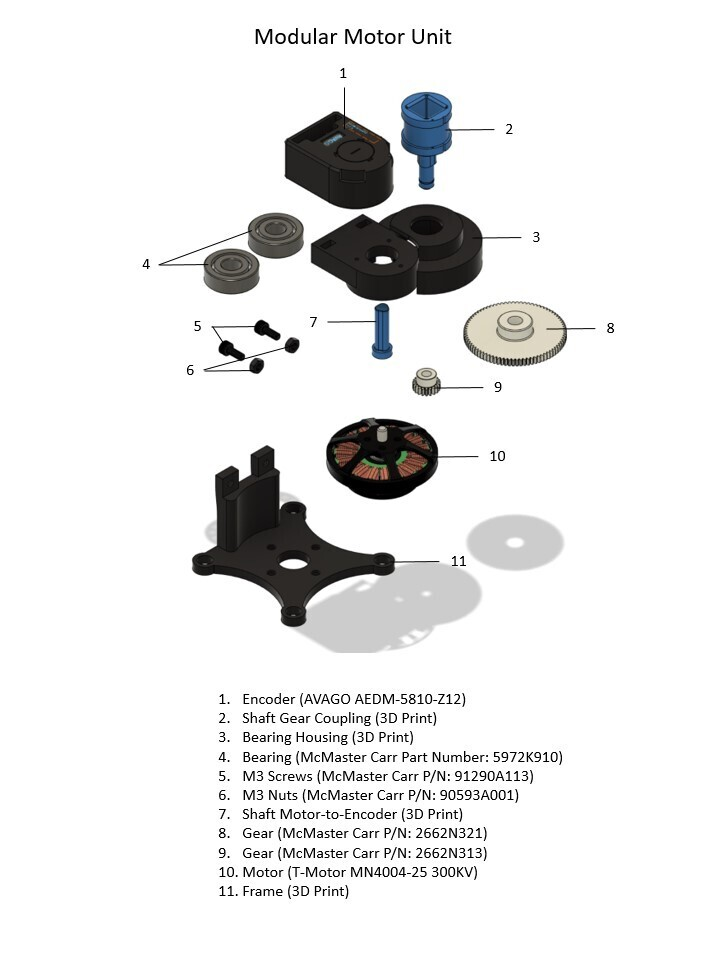
\includegraphics[width=\textwidth]{images/motor_unit.jpg}
    \caption{Complete schematic of the motor actuation unit, from \cite{motor_actuation_paper}}
    \label{fig:motor_unit}
\end{figure}

\paragraph{The workstation} used is a Dell OptiPlex 7090. It boasts an Intel Core i7-10700 CPU with 16GB of memory. It runs the RT-Preempt real time Linux kernel. The station communicates with the TI micro-controllers through a CAN-to-PCI Express interface card (IPEH-003027, PEAK system, Hessen, Germany). The station interfaces with the Aurora tracker through USB. Because the code for this thesis is written in Python, use of the real time kernel is not strictly required as Python does not support real time operations. For this project Python was deemed an appropriate language as it enables faster development times, and the shortcoming in terms of runtime is not seen to cause issues on the system. 

\subsubsection{Maximum Curvature Test}
Before the 16:1 gearbox was designed and installed, the actuation unit had a 4:1 gear ratio. An experiment was conducted to determine the arm length that enabled the largest range in the end effector position. Knowing the maximum and minimum distance that can be reached from an arm's base is required to set workspace bounds for the robot controller. The maximum distance is trivially given by the length of the arm. To find the minimum distance, a maximum curvature is applied by sending the highest current command a motor can support. The curvature that equates the bending forces to the maximum motor torque is taken as the maximum curvature. In this position, the distance between the end effector and arm base was measured. The results are displayed in Table \ref{tab:arm_length} and Figure \ref{fig:maximum_curve}. The arms were left at \SI{80}{cm} length as no notable gain in performance was observed at either test length. 

\begin{table}[h]
    \centering
    \caption{Arm distances during the maximum curvature test}
    \begin{tabular}{c|c|c}
        Extended Distance & Fully Contracted Distance & Contraction Distance \\
        \hline
        \SI{80}{cm} & \SI{59(1)}{cm} & \SI{21(1)}{cm} \\
        \SI{55}{cm} & \SI{33(1)}{cm} & \SI{22(1)}{cm} \\
    \end{tabular}
    \label{tab:arm_length}
\end{table}

This experiment showed the torque output of the motors resulted in a significantly smaller range of motion than what was initially expected. In response, a new gearbox was designed and manufactured to increase the maximum torque output of the robot. With the new gearbox, the robot is able to contract its arm completely with \SI{0}{cm} between the end effector and base. 

\begin{figure}[H]
     \centering
     \begin{subfigure}[b]{0.48\textwidth}
         \centering
         \includegraphics[width=\textwidth]{images/max_curve1.png}
         \caption{Without gearbox}
         \label{fig:maximum_curve1}
     \end{subfigure}
     \hfill
     \begin{subfigure}[b]{0.48\textwidth}
         \centering
         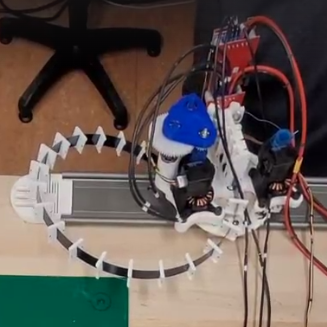
\includegraphics[width=\textwidth]{images/max_curve2.png}
         \caption{With gearbox}
         \label{fig:maximum_curve2}
     \end{subfigure}
        \caption{Maximum curvature tests}
        \label{fig:maximum_curve}
\end{figure}

